%pdflatex-../thesis.tex
% vim:spell spelllang=en_us

Themis is an application for evaluation of virtual machine migrations. It is prepared to be used for availability measurements and can be easily adjusted to perform other task during migration. 

Application is modular and can be adapted for different orchestrator or to perform different task during migration. Architecture is depicted in figure \ref{img:themis-model}. Backend is responsible for measurement management and results processing. Frontend provides web interface for users. Result can be displayed directly as table or graph in browser or exported into \Ac{CSV}.

\begin{figure}[htb]
	\begin{center}
	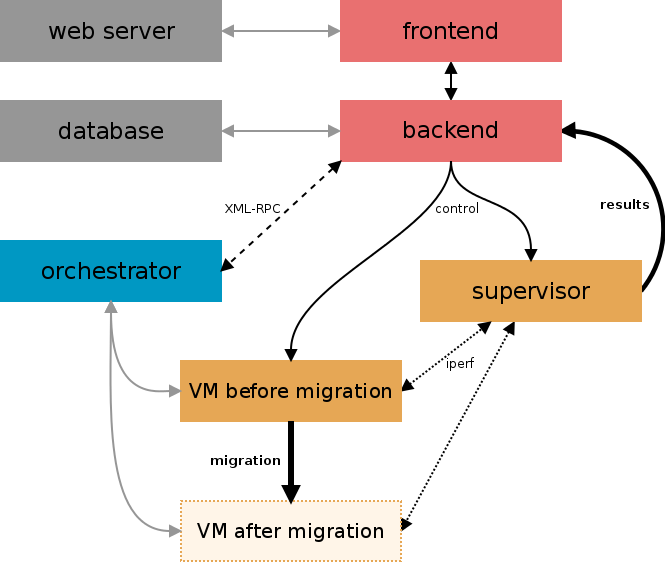
\includegraphics[width=0.7\textwidth]{themis-model.png}
	\end{center}
	\caption{Model of Themis application}
	\label{img:themis-model}
\end{figure}



% languages
Application is written in Ruby using Ruby on Rails framework. Ruby is platform independent and can run on every currently used operating system. Ruby on Rails (\Ac{RoR}) is framework providing database abstraction and strictly based on model-view-controller (\Ac{MVC}) architecture. Application is based on object model, outputs are generatied using views and controller is responsible for sending commands to models and forward results to views.

I have decided to use this framework because it provides better interaction with system services, e.g. \Ac{SSH} and \Ac{SCP}, than other web frameworks. There are public available classes for interaction with OpenNebula and OpenStack cloud \Ac{API} so it is not necessary to create \mbox{\Ac{XML}-\Ac{RPC}} parsers from scratch.

\section{Measure models}
There are three models defining measurement tasks and result. Definition, session and transfer. There models are used to describe migration tasks instructions, migration progress and results. 

All three models mentioned bellow are descendants of \Name{ActiveRecord::Base} and mapping between objects and tables is handled by this class. It also describes associations and perform validation.


\subsection{Definition}
Definition model, formally MeasureDefinition, is used to save prescription for measurement task. It is possible to crate definition in console or using web interface. Screenshot can be seen in figure \ref{img:web-new-definition}. 



\begin{description}
	\item[vm] is virtual machine which is going to be migrated, list of \Ac{VM}s available for migration is loaded on-demand from orchestrator using OneOrchestrator class. Virtual machine must be in running state and variable \Code{THEMIS\_TYPE = 'VM'} need to be present in contextualization settings.
	\item[source] is source host for virtual machine. \Ac{VM} need to be migrated to this host before starting measurement session. List of hosts is loaded using OneOrchestrator class and hosts status is checked for every hosts.
	\item[destination] is destination host. \Ac{VM} is migrated to this host during measurement session.
	\item[bandwidth] is determines packet generation rate passed to agent.
	\item[cycles] set number of migration repetitions.
	\item[supervisor] is an \Ac{IP} address of hypervisor node.
	\item[description] has an obvious meaning.

	\item[started\_at] is timestamp taken at the beginning of measurement.
	\item[finished\_at] is timestamp taken after finishing all migrations.
\end{description}

\begin{table}[htb]
\begin{center}
	\caption{MeasureDefinition parameters}
	\label{tab:measuredefinition-params}
	\begin{tabular}{|l|l|l|l|l|}
	\Th{Parameter} & \Th{Required} & \Th{Type} & \Th{User edit.} & \Th{Notes} \\
	vm & yes & string & yes & \\
	source & yes & integer & yes & \\
	destination & yes & integer & yes & \\
	bandwidth & yes & integer & yes & \\
	cycles & yes & integer & yes & \\
	supervisor & yes & string & yes & \Ac{IP} address \\ 
	description & no & text & yes & \\
	started\_at & no & timestamp & no & \\
	finished\_at & no & timestamp & no & \\
	\end{tabular}
\end{center}
\end{table}


% connection with orchestrator


\begin{figure}[htb]
	\begin{center}
	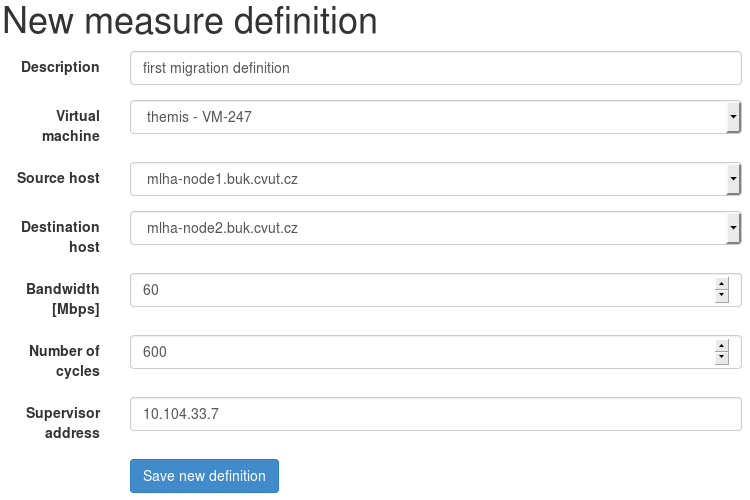
\includegraphics[width=0.9\textwidth]{form_measure_definition_new.png}
	\end{center}
	\caption{Web interface - new definition}
	\label{img:web-new-definition}
\end{figure}

	
\subsection{Session}

\subsection{Transfer}

% delayed job


\section{Virtual machines}

\section{Agent}
It was necessary to develop a script wrapper capable to parse iperf output and upload results to backend module. This script is called agent.rb, it is attached on on the CD and will be published in project repository. It is written in Ruby to be compatible with rest of the project. Agent script is executed from backend in migration\_session model in start method and \Ac{SSH} is used for remote execution.

Agent script need to be available in virtual machine under test as well as in hypervisor. However distribution is fairly simple because it is just a single file (agent.rb) with a few dependencies. This file can be distributed manually, which is not very usable for large or frequent deployment. Automatic deployment using OpenNebula's contextualization is much more efficient since orchestrator takes care of saving file into \Ac{VM}s. 
It is also possible to use configuration management system to upload this file and prepare environment to run migration. I have used Ansible to deploy agent.rb because it was necessary to update Ruby version. 

There are two modes of running agent. Modes differ in packet generator parameters and required dependencies. Mode is determined by \Code{ARGV[0]} parameter, which is the first parameter after filename. It is necessary select correct mode and properly configure all parameters from table \ref{tab:agent-parameters} because measure session can not be established otherwise. 

Generator mode only generates packets and sends them to receiver so it require nothing more than Ruby and iperf available. Receiver mode is more advanced and it uploads results to backend besides receiving packet. Receiver mode requires these dependencies:
\begin{itemize}
	\item \B{net/http} is used to upload results to backend using \Ac{HTTP} POST method
	\item \B{json} is necessary to export data into \Ac{JSON} before sending
	\item \B{date} is used to parse timestamp provided iperf and convert it into backend compatible format
\end{itemize}

% dependencies 
Both modes use IO class to read pipeline output from iperf program. This class is, however, part of Ruby core so it is not necessary to install it separately. Receriver dependencies can be install using distribution package manager or with gem utility using command \Cmd{gem install net/http json date}.

\begin{table}[htb]
\begin{center}
	\caption{Agent.rb paramaters}
	\label{tab:agent-parameters}
	\begin{tabularx}{\textwidth}{|r|l|l||l|X|}
	\multicolumn{3}{c}{\Th{Generator mode}} & \multicolumn{2}{c}{\Th{Receiver mode}} \\
	\hline
	\# & {Parameter} & {Example}  & {Parameter} & {Example} \\
	\hline
	\hline
	0 & Mode & generator & Mode & receiver \\
	\hline
	1 & Destination \Ac{IP} & 192.0.2.1 & Listen \Ac{IP} & 192.0.2.1 \\
	\hline
	2 & Destination port & 5004 & Listen port & 5004 \\
	\hline
	3 & Bandwidth & 1M & Upload \Ac{URL} & \url{http://backend/measure_transfers/23.json} \\
	\hline
	\end{tabularx}
\end{center}
\end{table}


% iperf crap
Agent is using legacy iperf version developed by NLANR/DAST but it introduces several problems which must be resolved in agent.rb and measure session routine. I am going to adapt agent.rb for iperf3\footnote{Available on \url{https://github.com/esnet/iperf}} which is new implementation developed by ESnet/Lawrence Berkeley National Laboratory. Iperf3 provides \Ac{JSON} output and probably will not suffer from problems presented below.

First problem is automatic session reestablishment. This occurs when running session is interrupted by a client and new session is initialized with the same receiver in short interval (less than few seconds). Iperf server joins new session with previous one which is not desired solution. This it the reason why there is 5 second interval inserted before generator restart. 

Second problem is handling INT signal by legacy iperf. SIGINT is reserved for external interrupt and this signal is for example sent to process when \mbox{Ctrl + C} is pressed. Iperf catches this signal preventing user to accidentally stop measure session. I understand reason why this function was implemented but I think that is total nonsense to require two consecutive INT signals to quit program. I have solved this by trapping SIGINT and sending KILL signal to iperf before agent.rb exit. This is only one possible way to reliably stop running agent together with iperf.

\begin{figure}[htb]
\caption{Example of agent.rb and iperf commands}
\label{code:fw}
\begin{verbatim}
# agent in generator mode
./agent.rb "generator" 192.0.2.1 5004 10M
# expanded iperf command in generator mode
iperf --udp --interval 1 --time 3600 --client 192.0.2.1 --port 5004 \
--bandwidth 10M --format b
	
# agent in receiver mode
./agent.rb "receiver" 192.0.2.1 5004 http://backend/measure_transfers/23.json
# expanded iperf command in receiver mode
iperf --server --bind 192.0.2.1 --port 5004 --udp --interval \
--reportstyle c --format
\end{verbatim}
\end{figure}


\section{Application}
	% backend
	% frontend
	% orchestrator
	% database
	% web server

	% měření pro elmag

